\begin{figure}[H]
\centering

\includegraphics[width=\textwidth]{实验报告9-2025051222.jpg}
% \caption{}
\label{}
\end{figure}

\section{作业}

\begin{figure}[H]
\centering
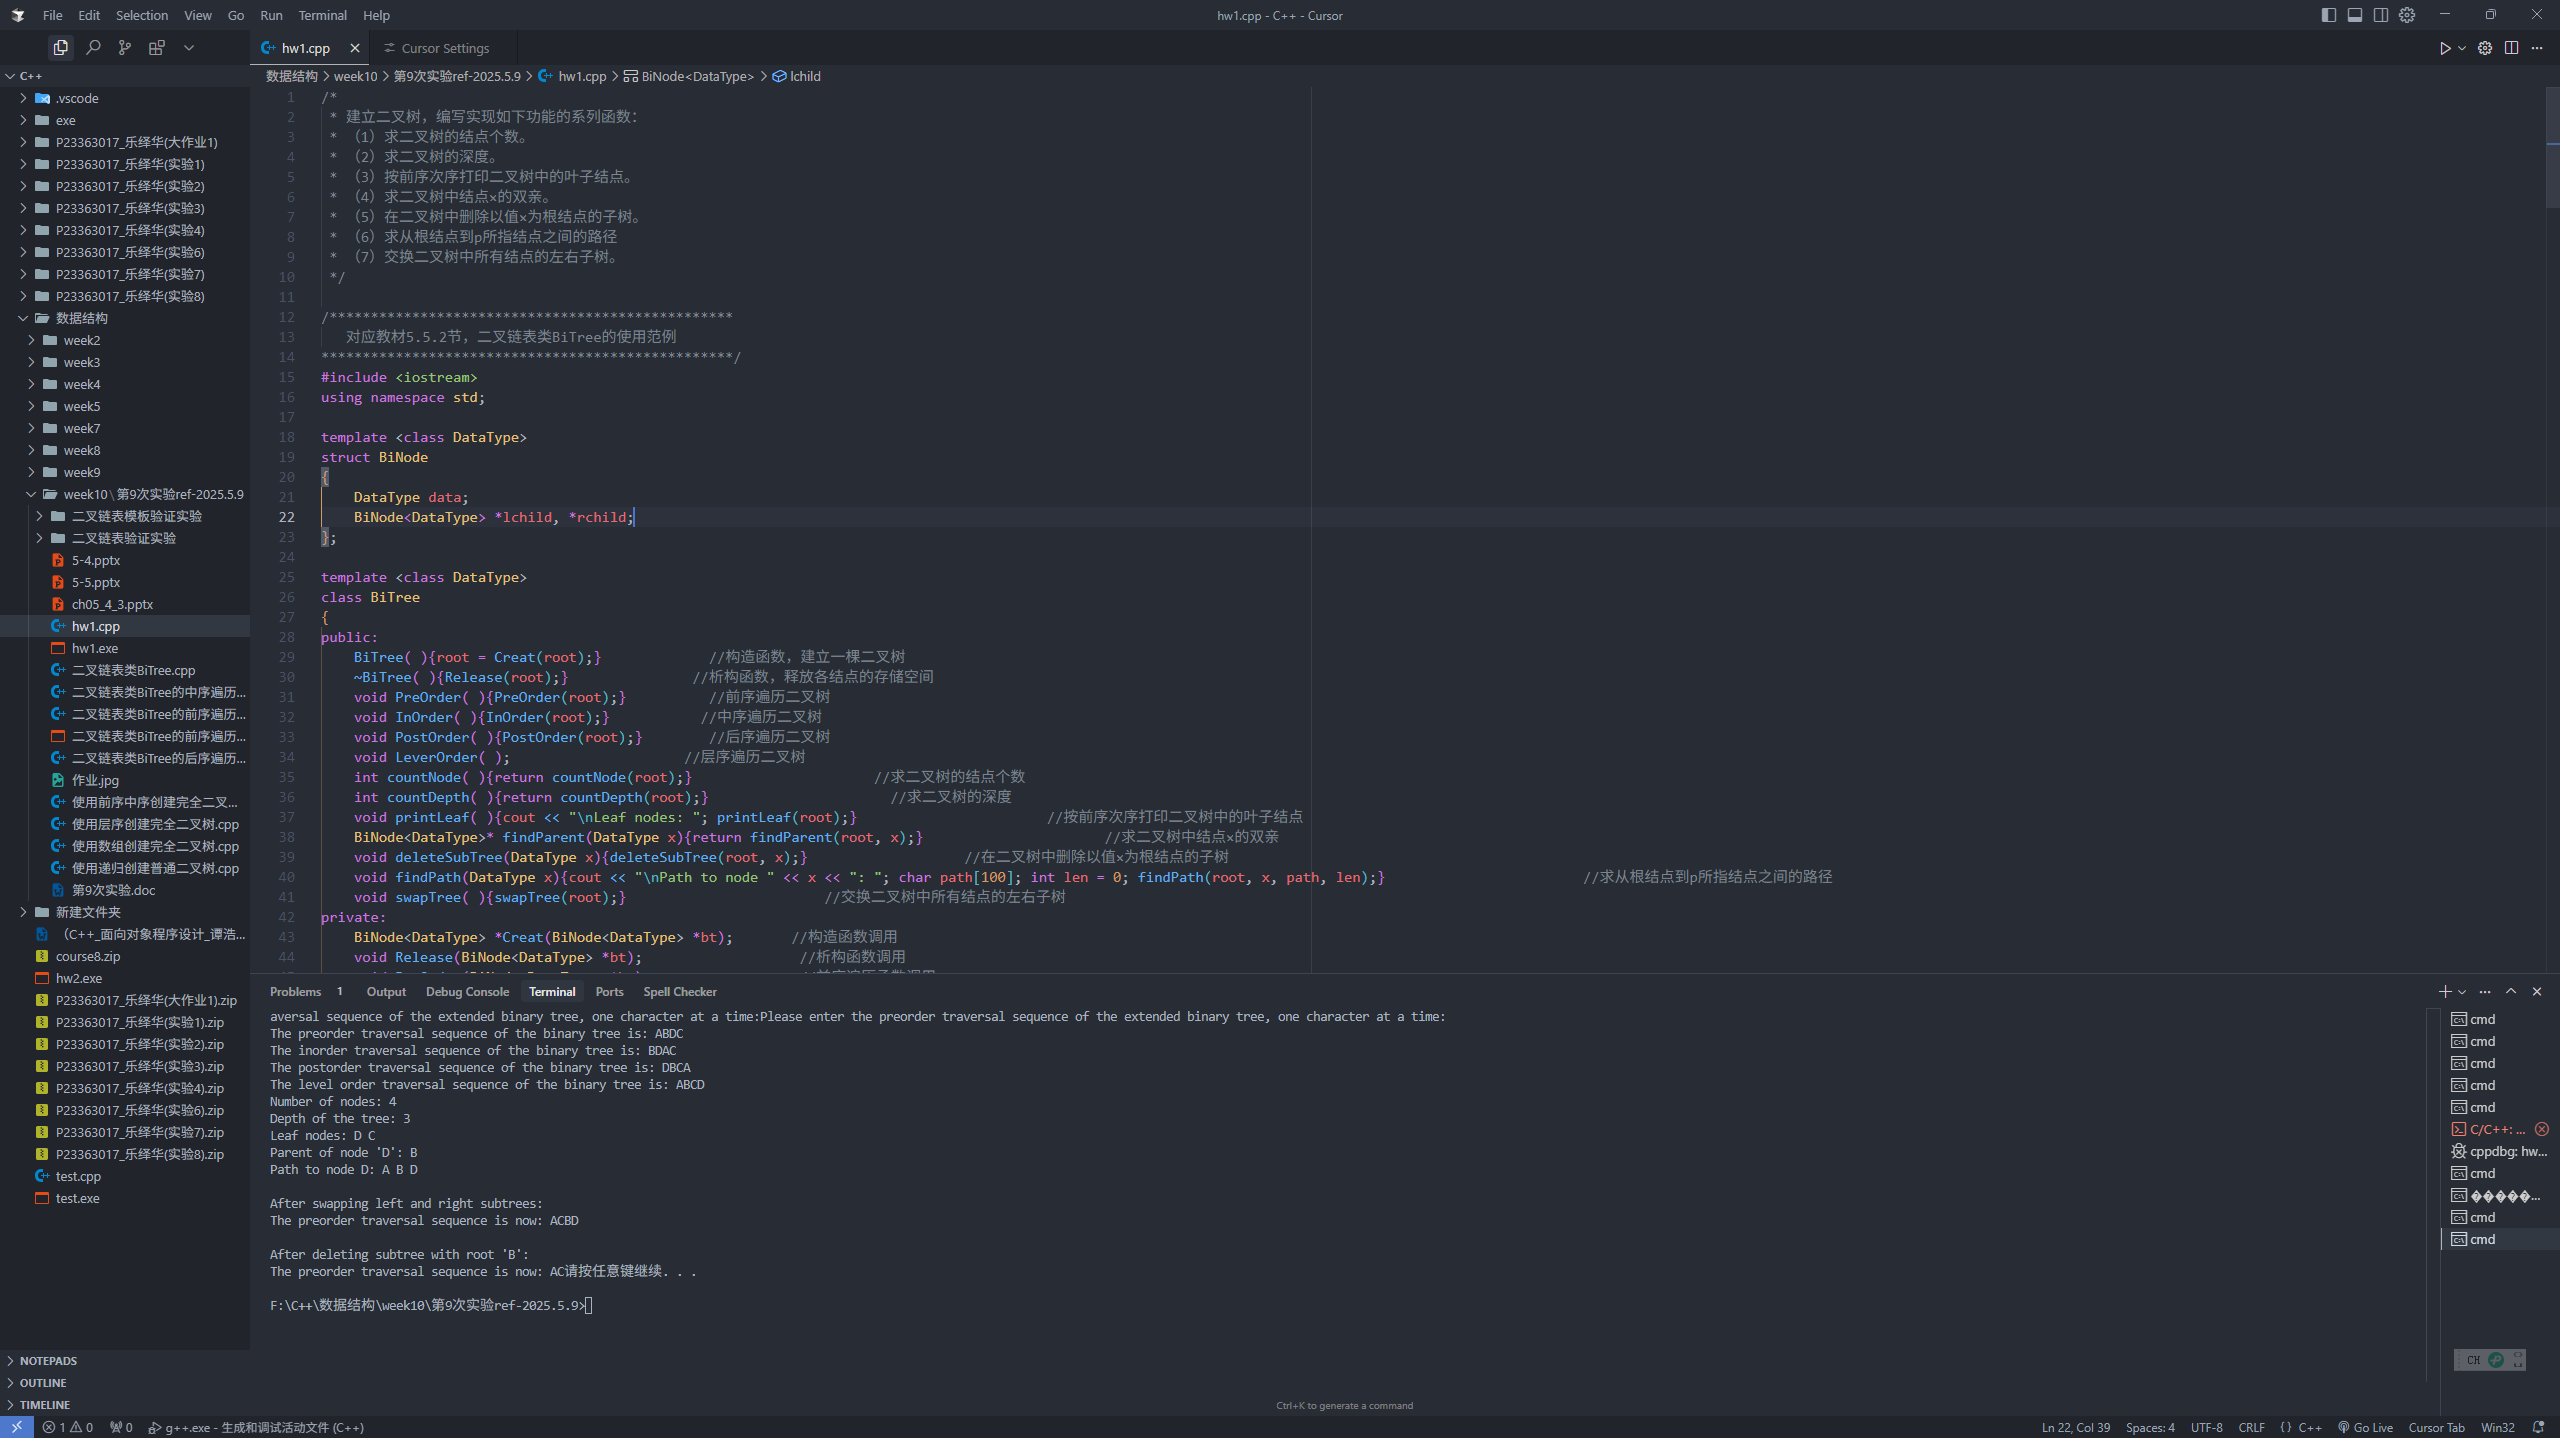
\includegraphics[width=\textwidth]{实验报告9-2025051222.png}
% \caption{}
\label{}
\end{figure}

\begin{lstlisting}[language=C++]
/*

 * 建立二叉树,编写实现如下功能的系列函数:

 * (1)求二叉树的结点个数。

 * (2)求二叉树的深度。

 * (3)按前序次序打印二叉树中的叶子结点。

 * (4)求二叉树中结点×的双亲。

 * (5)在二叉树中删除以值×为根结点的子树。

 * (6)求从根结点到p所指结点之间的路径

 * (7)交换二叉树中所有结点的左右子树。

 */

  

/*************************************************

   对应教材5.5.2节,二叉链表类BiTree的使用范例

**************************************************/

#include <iostream>

using namespace std;

  

template <class DataType>

struct BiNode

{

    DataType data;

    BiNode<DataType> *lchild, *rchild;

};

  

template <class DataType>

class BiTree

{

public:

    BiTree( ){root = Creat(root);}             //构造函数,建立一棵二叉树

    ~BiTree( ){Release(root);}               //析构函数,释放各结点的存储空间

    void PreOrder( ){PreOrder(root);}          //前序遍历二叉树

    void InOrder( ){InOrder(root);}           //中序遍历二叉树

    void PostOrder( ){PostOrder(root);}        //后序遍历二叉树

    void LeverOrder( );                     //层序遍历二叉树

    int countNode( ){return countNode(root);}                      //求二叉树的结点个数

    int countDepth( ){return countDepth(root);}                      //求二叉树的深度

    void printLeaf( ){cout << "\nLeaf nodes: "; printLeaf(root);}                       //按前序次序打印二叉树中的叶子结点

    BiNode<DataType>* findParent(DataType x){return findParent(root, x);}                      //求二叉树中结点×的双亲

    void deleteSubTree(DataType x){deleteSubTree(root, x);}                   //在二叉树中删除以值×为根结点的子树

    void findPath(DataType x){cout << "\nPath to node " << x << ": "; char path[100]; int len = 0; findPath(root, x, path, len);}                        //求从根结点到p所指结点之间的路径

    void swapTree( ){swapTree(root);}                        //交换二叉树中所有结点的左右子树

private:

    BiNode<DataType> *Creat(BiNode<DataType> *bt);       //构造函数调用

    void Release(BiNode<DataType> *bt);                   //析构函数调用

    void PreOrder(BiNode<DataType> *bt);                  //前序遍历函数调用

    void InOrder(BiNode<DataType> *bt);                   //中序遍历函数调用

    void PostOrder(BiNode<DataType> *bt);                 //后序遍历函数调用

    int countNode(BiNode<DataType> *bt);                //求二叉树的结点个数

    int countDepth(BiNode<DataType> *bt);              //求二叉树的深度

    void printLeaf(BiNode<DataType> *bt);              //按前序次序打印二叉树中的叶子结点

    BiNode<DataType>* findParent(BiNode<DataType> *bt, DataType x);             //求二叉树中结点×的双亲

    void deleteSubTree(BiNode<DataType> *&bt, DataType x);          //在二叉树中删除以值×为根结点的子树

    bool findPath(BiNode<DataType> *bt, DataType x, char path[], int &len);              //求从根结点到p所指结点之间的路径

    void swapTree(BiNode<DataType> *bt);              //交换二叉树中所有结点的左右子树

    BiNode<DataType> *root;                             //指向根结点的头指针

};

  

template <class DataType>

void BiTree<DataType> :: PreOrder(BiNode<DataType> *bt)

{

    if (bt == NULL) return;              //递归调用的结束条件

    else {

        cout << bt->data;                  //访问根结点bt的数据域

        PreOrder(bt->lchild);               //前序递归遍历bt的左子树

        PreOrder(bt->rchild);               //前序递归遍历bt的右子树  

    }

}

  

template <class DataType>

void BiTree<DataType> :: InOrder(BiNode<DataType> *bt)

{

    if (bt == NULL) return;              //递归调用的结束条件

    else {

        InOrder(bt->lchild);               //前序递归遍历bt的左子树

        cout << bt->data;                  //访问根结点bt的数据域

        InOrder(bt->rchild);               //前序递归遍历bt的右子树  

    }

}

  

template <class DataType>

void BiTree<DataType> :: PostOrder(BiNode<DataType> *bt)

{

    if (bt == NULL) return;              //递归调用的结束条件

    else {

        PostOrder(bt->lchild);               //前序递归遍历bt的左子树

        PostOrder(bt->rchild);               //前序递归遍历bt的右子树

        cout << bt->data;                  //访问根结点bt的数据域  

    }

}

  

template <class DataType>

void BiTree<DataType> :: LeverOrder( )

{

    BiNode<DataType> *Q[100], *q = NULL;      //顺序队列最多100个结点

    int front = -1, rear = -1;                      //队列初始化

    if (root == NULL) return;                    //二叉树为空,算法结束

    Q[++rear] = root;                           //根指针入队

    while (front != rear)          //当队列非空时

    {

        q = Q[++front];           //出队

        cout << q->data;  

        if (q->lchild != NULL)  Q[++rear] = q->lchild;

        if (q->rchild != NULL)  Q[++rear] = q->rchild;

    }  

}

  

template <class DataType>

BiNode<DataType> *BiTree<DataType> :: Creat(BiNode<DataType> *bt)

{

    char ch;

    cout << "Please enter the preorder traversal sequence of the extended binary tree, one character at a time:";

    //A B # D # # C # #

    cin >> ch;                      //输入结点的数据信息,假设为字符

    if (ch == '#') bt = NULL;                //建立一棵空树

    else {

        bt = new BiNode<DataType>; bt->data = ch;        

        bt->lchild = Creat(bt->lchild);          //递归建立左子树

        bt->rchild = Creat(bt->rchild);          //递归建立右子树

    }

    return bt;

}

  

template <class DataType>

void BiTree<DataType> :: Release(BiNode<DataType> *bt)

{

    if (bt == NULL) return;

    else{

        Release(bt->lchild);                   //释放左子树

        Release(bt->rchild);                   //释放右子树

        delete bt;                            //释放根结点

    }

}

  

template <class DataType>

int BiTree<DataType> :: countNode(BiNode<DataType> *bt)

{

    if (bt == NULL) return 0;              //递归调用的结束条件

    else {

        return 1 + countNode(bt->lchild) + countNode(bt->rchild);  //当前节点(1) + 左子树节点数 + 右子树节点数

    }

}

  

template <class DataType>

int BiTree<DataType> :: countDepth(BiNode<DataType> *bt)

{

    if (bt == NULL) return 0;              //递归调用的结束条件

    else {

        int leftDepth = countDepth(bt->lchild);

        int rightDepth = countDepth(bt->rchild);

        return (leftDepth > rightDepth ? leftDepth : rightDepth) + 1;  //较深子树深度 + 1

    }

}

  

template <class DataType>

void BiTree<DataType> :: printLeaf(BiNode<DataType> *bt)

{

    if (bt == NULL) return;              //递归调用的结束条件

    if (bt->lchild == NULL && bt->rchild == NULL) {

        cout << bt->data << " ";        //叶子结点,输出数据

    }

    printLeaf(bt->lchild);               //前序递归遍历bt的左子树

    printLeaf(bt->rchild);               //前序递归遍历bt的右子树

}

  

template <class DataType>

BiNode<DataType>* BiTree<DataType> :: findParent(BiNode<DataType> *bt, DataType x)

{

    if (bt == NULL || (bt->lchild == NULL && bt->rchild == NULL)) return NULL;

    // 检查左右子节点是否为目标值

    if ((bt->lchild != NULL && bt->lchild->data == x) ||

        (bt->rchild != NULL && bt->rchild->data == x)) {

        return bt;  // 当前节点是x的父节点

    }

    // 递归查找左右子树

    BiNode<DataType> *parent = findParent(bt->lchild, x);

    if (parent != NULL) return parent;

    return findParent(bt->rchild, x);

}

  

template <class DataType>

void BiTree<DataType> :: deleteSubTree(BiNode<DataType> *&bt, DataType x)

{

    if (bt == NULL) return;

    // 如果当前节点是要删除的子树根节点

    if (bt->data == x) {

        Release(bt);  // 释放整个子树

        bt = NULL;    // 将节点置为NULL

        return;

    }

    // 递归查找左右子树

    deleteSubTree(bt->lchild, x);

    deleteSubTree(bt->rchild, x);

}

  

template <class DataType>

bool BiTree<DataType> :: findPath(BiNode<DataType> *bt, DataType x, char path[], int &len)

{

    if (bt == NULL) return false;

    // 将当前节点添加到路径

    path[len++] = bt->data;

    // 找到目标节点

    if (bt->data == x) {

        for (int i = 0; i < len; i++) {

            cout << path[i] << " ";

        }

        return true;

    }

    // 递归查找左右子树

    if (findPath(bt->lchild, x, path, len) || findPath(bt->rchild, x, path, len)) {

        return true;  // 找到路径

    }

    // 回溯,当前路径不包含目标节点

    len--;

    return false;

}

  

template <class DataType>

void BiTree<DataType> :: swapTree(BiNode<DataType> *bt)

{

    if (bt == NULL) return;

    // 交换左右子树

    BiNode<DataType> *temp = bt->lchild;

    bt->lchild = bt->rchild;

    bt->rchild = temp;

    // 递归交换子树的左右子节点

    swapTree(bt->lchild);

    swapTree(bt->rchild);

}

  

int main(int argc, char* argv[])

{   // A B # D # # C # #

    BiTree<char> T;                           // Define object variable T

    cout << "\nThe preorder traversal sequence of the binary tree is: ";

    T.PreOrder();

    cout << "\nThe inorder traversal sequence of the binary tree is: ";

    T.InOrder();

    cout << "\nThe postorder traversal sequence of the binary tree is: ";

    T.PostOrder();

    cout << "\nThe level order traversal sequence of the binary tree is: ";

    T.LeverOrder();

    cout << "\nNumber of nodes: " << T.countNode();

    cout << "\nDepth of the tree: " << T.countDepth();

    T.printLeaf();

    cout << "\nParent of node 'D': ";

    BiNode<char> *parent = T.findParent('D');

    if (parent != NULL) cout << parent->data;

    else cout << "Not found";

    T.findPath('D');

    cout << "\n\nAfter swapping left and right subtrees:";

    T.swapTree();

    cout << "\nThe preorder traversal sequence is now: ";

    T.PreOrder();

    T.deleteSubTree('B');

    cout << "\n\nAfter deleting subtree with root 'B':";

    cout << "\nThe preorder traversal sequence is now: ";

    T.PreOrder();

    system("pause");  // 让控制台窗口保持打开状态

    return 0;

}
\end{lstlisting}